\documentclass{article}
\usepackage{graphicx}
\usepackage{geometry}
\usepackage{amsmath}
\usepackage{float}
\usepackage{xcolor}
\usepackage{listings}
\usepackage{caption}
\usepackage{subcaption}
\usepackage{xparse}
\usepackage{hyperref}
\usepackage{fancyhdr}
\pagestyle{fancy}
 %%%%%%%%%%%%%%%%%%%%%%%%%%%%%%%%%%%%%%%%%%%%%%%%%%%%%%%%%%%%%%%%%%%%%%%%%%%%%%%% 
%%% ~ Arduino Language - Arduino IDE Colors ~                                  %%%
%%%                                                                            %%%
%%% Kyle Rocha-Brownell | 10/2/2017 | No Licence                               %%%
%%% -------------------------------------------------------------------------- %%%
%%%                                                                            %%%
%%% Place this file in your working directory (next to the latex file you're   %%%
%%% working on).  To add it to your project, place:                            %%%
%%%     %%%%%%%%%%%%%%%%%%%%%%%%%%%%%%%%%%%%%%%%%%%%%%%%%%%%%%%%%%%%%%%%%%%%%%%%%%%%%%%% 
%%% ~ Arduino Language - Arduino IDE Colors ~                                  %%%
%%%                                                                            %%%
%%% Kyle Rocha-Brownell | 10/2/2017 | No Licence                               %%%
%%% -------------------------------------------------------------------------- %%%
%%%                                                                            %%%
%%% Place this file in your working directory (next to the latex file you're   %%%
%%% working on).  To add it to your project, place:                            %%%
%%%     %%%%%%%%%%%%%%%%%%%%%%%%%%%%%%%%%%%%%%%%%%%%%%%%%%%%%%%%%%%%%%%%%%%%%%%%%%%%%%%% 
%%% ~ Arduino Language - Arduino IDE Colors ~                                  %%%
%%%                                                                            %%%
%%% Kyle Rocha-Brownell | 10/2/2017 | No Licence                               %%%
%%% -------------------------------------------------------------------------- %%%
%%%                                                                            %%%
%%% Place this file in your working directory (next to the latex file you're   %%%
%%% working on).  To add it to your project, place:                            %%%
%%%    \input{arduinoLanguage.tex}                                             %%%
%%% somewhere before \begin{document} in your latex file.                      %%%
%%%                                                                            %%%
%%% In your document, place your arduino code between:                         %%%
%%%   \begin{lstlisting}[language=Arduino]                                     %%%
%%% and:                                                                       %%%
%%%   \end{lstlisting}                                                         %%%
%%%                                                                            %%%
%%% Or create your own style to add non-built-in functions and variables.      %%%
%%%                                                                            %%%
 %%%%%%%%%%%%%%%%%%%%%%%%%%%%%%%%%%%%%%%%%%%%%%%%%%%%%%%%%%%%%%%%%%%%%%%%%%%%%%%% 

\usepackage{color}
\usepackage{listings}    
\usepackage{courier}

%%% Define Custom IDE Colors %%%
\definecolor{arduinoGreen}    {rgb} {0.17, 0.43, 0.01}
\definecolor{arduinoGrey}     {rgb} {0.47, 0.47, 0.33}
\definecolor{arduinoOrange}   {rgb} {0.8 , 0.4 , 0   }
\definecolor{arduinoBlue}     {rgb} {0.01, 0.61, 0.98}
\definecolor{arduinoDarkBlue} {rgb} {0.0 , 0.2 , 0.5 }

%%% Define Arduino Language %%%
\lstdefinelanguage{Arduino}{
  language=C++, % begin with default C++ settings 
%
%
  %%% Keyword Color Group 1 %%%  (called KEYWORD3 by arduino)
  keywordstyle=\color{arduinoGreen},   
  deletekeywords={  % remove all arduino keywords that might be in c++
                break, case, override, final, continue, default, do, else, for, 
                if, return, goto, switch, throw, try, while, setup, loop, export, 
                not, or, and, xor, include, define, elif, else, error, if, ifdef, 
                ifndef, pragma, warning,
                HIGH, LOW, INPUT, INPUT_PULLUP, OUTPUT, DEC, BIN, HEX, OCT, PI, 
                HALF_PI, TWO_PI, LSBFIRST, MSBFIRST, CHANGE, FALLING, RISING, 
                DEFAULT, EXTERNAL, INTERNAL, INTERNAL1V1, INTERNAL2V56, LED_BUILTIN, 
                LED_BUILTIN_RX, LED_BUILTIN_TX, DIGITAL_MESSAGE, FIRMATA_STRING, 
                ANALOG_MESSAGE, REPORT_DIGITAL, REPORT_ANALOG, SET_PIN_MODE, 
                SYSTEM_RESET, SYSEX_START, auto, int8_t, int16_t, int32_t, int64_t, 
                uint8_t, uint16_t, uint32_t, uint64_t, char16_t, char32_t, operator, 
                enum, delete, bool, boolean, byte, char, const, false, float, double, 
                null, NULL, int, long, new, private, protected, public, short, 
                signed, static, volatile, String, void, true, unsigned, word, array, 
                sizeof, dynamic_cast, typedef, const_cast, struct, static_cast, union, 
                friend, extern, class, reinterpret_cast, register, explicit, inline, 
                _Bool, complex, _Complex, _Imaginary, atomic_bool, atomic_char, 
                atomic_schar, atomic_uchar, atomic_short, atomic_ushort, atomic_int, 
                atomic_uint, atomic_long, atomic_ulong, atomic_llong, atomic_ullong, 
                virtual, PROGMEM,
                Serial, Serial1, Serial2, Serial3, SerialUSB, Keyboard, Mouse,
                abs, acos, asin, atan, atan2, ceil, constrain, cos, degrees, exp, 
                floor, log, map, max, min, radians, random, randomSeed, round, sin, 
                sq, sqrt, tan, pow, bitRead, bitWrite, bitSet, bitClear, bit, 
                highByte, lowByte, analogReference, analogRead, 
                analogReadResolution, analogWrite, analogWriteResolution, 
                attachInterrupt, detachInterrupt, digitalPinToInterrupt, delay, 
                delayMicroseconds, digitalWrite, digitalRead, interrupts, millis, 
                micros, noInterrupts, noTone, pinMode, pulseIn, pulseInLong, shiftIn, 
                shiftOut, tone, yield, Stream, begin, end, peek, read, print, 
                println, available, availableForWrite, flush, setTimeout, find, 
                findUntil, parseInt, parseFloat, readBytes, readBytesUntil, readString, 
                readStringUntil, trim, toUpperCase, toLowerCase, charAt, compareTo, 
                concat, endsWith, startsWith, equals, equalsIgnoreCase, getBytes, 
                indexOf, lastIndexOf, length, replace, setCharAt, substring, 
                toCharArray, toInt, press, release, releaseAll, accept, click, move, 
                isPressed, isAlphaNumeric, isAlpha, isAscii, isWhitespace, isControl, 
                isDigit, isGraph, isLowerCase, isPrintable, isPunct, isSpace, 
                isUpperCase, isHexadecimalDigit, 
                }, 
  morekeywords={   % add arduino structures to group 1
                break, case, override, final, continue, default, do, else, for, 
                if, return, goto, switch, throw, try, while, setup, loop, export, 
                not, or, and, xor, include, define, elif, else, error, if, ifdef, 
                ifndef, pragma, warning,
                }, 
% 
%
  %%% Keyword Color Group 2 %%%  (called LITERAL1 by arduino)
  keywordstyle=[2]\color{arduinoBlue},   
  keywords=[2]{   % add variables and dataTypes as 2nd group  
                HIGH, LOW, INPUT, INPUT_PULLUP, OUTPUT, DEC, BIN, HEX, OCT, PI, 
                HALF_PI, TWO_PI, LSBFIRST, MSBFIRST, CHANGE, FALLING, RISING, 
                DEFAULT, EXTERNAL, INTERNAL, INTERNAL1V1, INTERNAL2V56, LED_BUILTIN, 
                LED_BUILTIN_RX, LED_BUILTIN_TX, DIGITAL_MESSAGE, FIRMATA_STRING, 
                ANALOG_MESSAGE, REPORT_DIGITAL, REPORT_ANALOG, SET_PIN_MODE, 
                SYSTEM_RESET, SYSEX_START, auto, int8_t, int16_t, int32_t, int64_t, 
                uint8_t, uint16_t, uint32_t, uint64_t, char16_t, char32_t, operator, 
                enum, delete, bool, boolean, byte, char, const, false, float, double, 
                null, NULL, int, long, new, private, protected, public, short, 
                signed, static, volatile, String, void, true, unsigned, word, array, 
                sizeof, dynamic_cast, typedef, const_cast, struct, static_cast, union, 
                friend, extern, class, reinterpret_cast, register, explicit, inline, 
                _Bool, complex, _Complex, _Imaginary, atomic_bool, atomic_char, 
                atomic_schar, atomic_uchar, atomic_short, atomic_ushort, atomic_int, 
                atomic_uint, atomic_long, atomic_ulong, atomic_llong, atomic_ullong, 
                virtual, PROGMEM,
                },  
% 
%
  %%% Keyword Color Group 3 %%%  (called KEYWORD1 by arduino)
  keywordstyle=[3]\bfseries\color{arduinoOrange},
  keywords=[3]{  % add built-in functions as a 3rd group
                Serial, Serial1, Serial2, Serial3, SerialUSB, Keyboard, Mouse,
                },      
%
%
  %%% Keyword Color Group 4 %%%  (called KEYWORD2 by arduino)
  keywordstyle=[4]\color{arduinoOrange},
  keywords=[4]{  % add more built-in functions as a 4th group
                abs, acos, asin, atan, atan2, ceil, constrain, cos, degrees, exp, 
                floor, log, map, max, min, radians, random, randomSeed, round, sin, 
                sq, sqrt, tan, pow, bitRead, bitWrite, bitSet, bitClear, bit, 
                highByte, lowByte, analogReference, analogRead, 
                analogReadResolution, analogWrite, analogWriteResolution, 
                attachInterrupt, detachInterrupt, digitalPinToInterrupt, delay, 
                delayMicroseconds, digitalWrite, digitalRead, interrupts, millis, 
                micros, noInterrupts, noTone, pinMode, pulseIn, pulseInLong, shiftIn, 
                shiftOut, tone, yield, Stream, begin, end, peek, read, print, 
                println, available, availableForWrite, flush, setTimeout, find, 
                findUntil, parseInt, parseFloat, readBytes, readBytesUntil, readString, 
                readStringUntil, trim, toUpperCase, toLowerCase, charAt, compareTo, 
                concat, endsWith, startsWith, equals, equalsIgnoreCase, getBytes, 
                indexOf, lastIndexOf, length, replace, setCharAt, substring, 
                toCharArray, toInt, press, release, releaseAll, accept, click, move, 
                isPressed, isAlphaNumeric, isAlpha, isAscii, isWhitespace, isControl, 
                isDigit, isGraph, isLowerCase, isPrintable, isPunct, isSpace, 
                isUpperCase, isHexadecimalDigit, 
                },      
%
%
  %%% Set Other Colors %%%
  stringstyle=\color{arduinoDarkBlue},    
  commentstyle=\color{arduinoGrey},    
%          
%   
  %%%% Line Numbering %%%%
   numbers=left,                    
  numbersep=5pt,                   
  numberstyle=\color{arduinoGrey},    
  %stepnumber=2,                      % show every 2 line numbers
%
%
  %%%% Code Box Style %%%%
  breaklines=true,                    % wordwrapping
  frame=shadowbox,
  tabsize=2,         
  basicstyle=\ttfamily  
}                                             %%%
%%% somewhere before \begin{document} in your latex file.                      %%%
%%%                                                                            %%%
%%% In your document, place your arduino code between:                         %%%
%%%   \begin{lstlisting}[language=Arduino]                                     %%%
%%% and:                                                                       %%%
%%%   \end{lstlisting}                                                         %%%
%%%                                                                            %%%
%%% Or create your own style to add non-built-in functions and variables.      %%%
%%%                                                                            %%%
 %%%%%%%%%%%%%%%%%%%%%%%%%%%%%%%%%%%%%%%%%%%%%%%%%%%%%%%%%%%%%%%%%%%%%%%%%%%%%%%% 

\usepackage{color}
\usepackage{listings}    
\usepackage{courier}

%%% Define Custom IDE Colors %%%
\definecolor{arduinoGreen}    {rgb} {0.17, 0.43, 0.01}
\definecolor{arduinoGrey}     {rgb} {0.47, 0.47, 0.33}
\definecolor{arduinoOrange}   {rgb} {0.8 , 0.4 , 0   }
\definecolor{arduinoBlue}     {rgb} {0.01, 0.61, 0.98}
\definecolor{arduinoDarkBlue} {rgb} {0.0 , 0.2 , 0.5 }

%%% Define Arduino Language %%%
\lstdefinelanguage{Arduino}{
  language=C++, % begin with default C++ settings 
%
%
  %%% Keyword Color Group 1 %%%  (called KEYWORD3 by arduino)
  keywordstyle=\color{arduinoGreen},   
  deletekeywords={  % remove all arduino keywords that might be in c++
                break, case, override, final, continue, default, do, else, for, 
                if, return, goto, switch, throw, try, while, setup, loop, export, 
                not, or, and, xor, include, define, elif, else, error, if, ifdef, 
                ifndef, pragma, warning,
                HIGH, LOW, INPUT, INPUT_PULLUP, OUTPUT, DEC, BIN, HEX, OCT, PI, 
                HALF_PI, TWO_PI, LSBFIRST, MSBFIRST, CHANGE, FALLING, RISING, 
                DEFAULT, EXTERNAL, INTERNAL, INTERNAL1V1, INTERNAL2V56, LED_BUILTIN, 
                LED_BUILTIN_RX, LED_BUILTIN_TX, DIGITAL_MESSAGE, FIRMATA_STRING, 
                ANALOG_MESSAGE, REPORT_DIGITAL, REPORT_ANALOG, SET_PIN_MODE, 
                SYSTEM_RESET, SYSEX_START, auto, int8_t, int16_t, int32_t, int64_t, 
                uint8_t, uint16_t, uint32_t, uint64_t, char16_t, char32_t, operator, 
                enum, delete, bool, boolean, byte, char, const, false, float, double, 
                null, NULL, int, long, new, private, protected, public, short, 
                signed, static, volatile, String, void, true, unsigned, word, array, 
                sizeof, dynamic_cast, typedef, const_cast, struct, static_cast, union, 
                friend, extern, class, reinterpret_cast, register, explicit, inline, 
                _Bool, complex, _Complex, _Imaginary, atomic_bool, atomic_char, 
                atomic_schar, atomic_uchar, atomic_short, atomic_ushort, atomic_int, 
                atomic_uint, atomic_long, atomic_ulong, atomic_llong, atomic_ullong, 
                virtual, PROGMEM,
                Serial, Serial1, Serial2, Serial3, SerialUSB, Keyboard, Mouse,
                abs, acos, asin, atan, atan2, ceil, constrain, cos, degrees, exp, 
                floor, log, map, max, min, radians, random, randomSeed, round, sin, 
                sq, sqrt, tan, pow, bitRead, bitWrite, bitSet, bitClear, bit, 
                highByte, lowByte, analogReference, analogRead, 
                analogReadResolution, analogWrite, analogWriteResolution, 
                attachInterrupt, detachInterrupt, digitalPinToInterrupt, delay, 
                delayMicroseconds, digitalWrite, digitalRead, interrupts, millis, 
                micros, noInterrupts, noTone, pinMode, pulseIn, pulseInLong, shiftIn, 
                shiftOut, tone, yield, Stream, begin, end, peek, read, print, 
                println, available, availableForWrite, flush, setTimeout, find, 
                findUntil, parseInt, parseFloat, readBytes, readBytesUntil, readString, 
                readStringUntil, trim, toUpperCase, toLowerCase, charAt, compareTo, 
                concat, endsWith, startsWith, equals, equalsIgnoreCase, getBytes, 
                indexOf, lastIndexOf, length, replace, setCharAt, substring, 
                toCharArray, toInt, press, release, releaseAll, accept, click, move, 
                isPressed, isAlphaNumeric, isAlpha, isAscii, isWhitespace, isControl, 
                isDigit, isGraph, isLowerCase, isPrintable, isPunct, isSpace, 
                isUpperCase, isHexadecimalDigit, 
                }, 
  morekeywords={   % add arduino structures to group 1
                break, case, override, final, continue, default, do, else, for, 
                if, return, goto, switch, throw, try, while, setup, loop, export, 
                not, or, and, xor, include, define, elif, else, error, if, ifdef, 
                ifndef, pragma, warning,
                }, 
% 
%
  %%% Keyword Color Group 2 %%%  (called LITERAL1 by arduino)
  keywordstyle=[2]\color{arduinoBlue},   
  keywords=[2]{   % add variables and dataTypes as 2nd group  
                HIGH, LOW, INPUT, INPUT_PULLUP, OUTPUT, DEC, BIN, HEX, OCT, PI, 
                HALF_PI, TWO_PI, LSBFIRST, MSBFIRST, CHANGE, FALLING, RISING, 
                DEFAULT, EXTERNAL, INTERNAL, INTERNAL1V1, INTERNAL2V56, LED_BUILTIN, 
                LED_BUILTIN_RX, LED_BUILTIN_TX, DIGITAL_MESSAGE, FIRMATA_STRING, 
                ANALOG_MESSAGE, REPORT_DIGITAL, REPORT_ANALOG, SET_PIN_MODE, 
                SYSTEM_RESET, SYSEX_START, auto, int8_t, int16_t, int32_t, int64_t, 
                uint8_t, uint16_t, uint32_t, uint64_t, char16_t, char32_t, operator, 
                enum, delete, bool, boolean, byte, char, const, false, float, double, 
                null, NULL, int, long, new, private, protected, public, short, 
                signed, static, volatile, String, void, true, unsigned, word, array, 
                sizeof, dynamic_cast, typedef, const_cast, struct, static_cast, union, 
                friend, extern, class, reinterpret_cast, register, explicit, inline, 
                _Bool, complex, _Complex, _Imaginary, atomic_bool, atomic_char, 
                atomic_schar, atomic_uchar, atomic_short, atomic_ushort, atomic_int, 
                atomic_uint, atomic_long, atomic_ulong, atomic_llong, atomic_ullong, 
                virtual, PROGMEM,
                },  
% 
%
  %%% Keyword Color Group 3 %%%  (called KEYWORD1 by arduino)
  keywordstyle=[3]\bfseries\color{arduinoOrange},
  keywords=[3]{  % add built-in functions as a 3rd group
                Serial, Serial1, Serial2, Serial3, SerialUSB, Keyboard, Mouse,
                },      
%
%
  %%% Keyword Color Group 4 %%%  (called KEYWORD2 by arduino)
  keywordstyle=[4]\color{arduinoOrange},
  keywords=[4]{  % add more built-in functions as a 4th group
                abs, acos, asin, atan, atan2, ceil, constrain, cos, degrees, exp, 
                floor, log, map, max, min, radians, random, randomSeed, round, sin, 
                sq, sqrt, tan, pow, bitRead, bitWrite, bitSet, bitClear, bit, 
                highByte, lowByte, analogReference, analogRead, 
                analogReadResolution, analogWrite, analogWriteResolution, 
                attachInterrupt, detachInterrupt, digitalPinToInterrupt, delay, 
                delayMicroseconds, digitalWrite, digitalRead, interrupts, millis, 
                micros, noInterrupts, noTone, pinMode, pulseIn, pulseInLong, shiftIn, 
                shiftOut, tone, yield, Stream, begin, end, peek, read, print, 
                println, available, availableForWrite, flush, setTimeout, find, 
                findUntil, parseInt, parseFloat, readBytes, readBytesUntil, readString, 
                readStringUntil, trim, toUpperCase, toLowerCase, charAt, compareTo, 
                concat, endsWith, startsWith, equals, equalsIgnoreCase, getBytes, 
                indexOf, lastIndexOf, length, replace, setCharAt, substring, 
                toCharArray, toInt, press, release, releaseAll, accept, click, move, 
                isPressed, isAlphaNumeric, isAlpha, isAscii, isWhitespace, isControl, 
                isDigit, isGraph, isLowerCase, isPrintable, isPunct, isSpace, 
                isUpperCase, isHexadecimalDigit, 
                },      
%
%
  %%% Set Other Colors %%%
  stringstyle=\color{arduinoDarkBlue},    
  commentstyle=\color{arduinoGrey},    
%          
%   
  %%%% Line Numbering %%%%
   numbers=left,                    
  numbersep=5pt,                   
  numberstyle=\color{arduinoGrey},    
  %stepnumber=2,                      % show every 2 line numbers
%
%
  %%%% Code Box Style %%%%
  breaklines=true,                    % wordwrapping
  frame=shadowbox,
  tabsize=2,         
  basicstyle=\ttfamily  
}                                             %%%
%%% somewhere before \begin{document} in your latex file.                      %%%
%%%                                                                            %%%
%%% In your document, place your arduino code between:                         %%%
%%%   \begin{lstlisting}[language=Arduino]                                     %%%
%%% and:                                                                       %%%
%%%   \end{lstlisting}                                                         %%%
%%%                                                                            %%%
%%% Or create your own style to add non-built-in functions and variables.      %%%
%%%                                                                            %%%
 %%%%%%%%%%%%%%%%%%%%%%%%%%%%%%%%%%%%%%%%%%%%%%%%%%%%%%%%%%%%%%%%%%%%%%%%%%%%%%%% 

\usepackage{color}
\usepackage{listings}    
\usepackage{courier}

%%% Define Custom IDE Colors %%%
\definecolor{arduinoGreen}    {rgb} {0.17, 0.43, 0.01}
\definecolor{arduinoGrey}     {rgb} {0.47, 0.47, 0.33}
\definecolor{arduinoOrange}   {rgb} {0.8 , 0.4 , 0   }
\definecolor{arduinoBlue}     {rgb} {0.01, 0.61, 0.98}
\definecolor{arduinoDarkBlue} {rgb} {0.0 , 0.2 , 0.5 }

%%% Define Arduino Language %%%
\lstdefinelanguage{Arduino}{
  language=C++, % begin with default C++ settings 
%
%
  %%% Keyword Color Group 1 %%%  (called KEYWORD3 by arduino)
  keywordstyle=\color{arduinoGreen},   
  deletekeywords={  % remove all arduino keywords that might be in c++
                break, case, override, final, continue, default, do, else, for, 
                if, return, goto, switch, throw, try, while, setup, loop, export, 
                not, or, and, xor, include, define, elif, else, error, if, ifdef, 
                ifndef, pragma, warning,
                HIGH, LOW, INPUT, INPUT_PULLUP, OUTPUT, DEC, BIN, HEX, OCT, PI, 
                HALF_PI, TWO_PI, LSBFIRST, MSBFIRST, CHANGE, FALLING, RISING, 
                DEFAULT, EXTERNAL, INTERNAL, INTERNAL1V1, INTERNAL2V56, LED_BUILTIN, 
                LED_BUILTIN_RX, LED_BUILTIN_TX, DIGITAL_MESSAGE, FIRMATA_STRING, 
                ANALOG_MESSAGE, REPORT_DIGITAL, REPORT_ANALOG, SET_PIN_MODE, 
                SYSTEM_RESET, SYSEX_START, auto, int8_t, int16_t, int32_t, int64_t, 
                uint8_t, uint16_t, uint32_t, uint64_t, char16_t, char32_t, operator, 
                enum, delete, bool, boolean, byte, char, const, false, float, double, 
                null, NULL, int, long, new, private, protected, public, short, 
                signed, static, volatile, String, void, true, unsigned, word, array, 
                sizeof, dynamic_cast, typedef, const_cast, struct, static_cast, union, 
                friend, extern, class, reinterpret_cast, register, explicit, inline, 
                _Bool, complex, _Complex, _Imaginary, atomic_bool, atomic_char, 
                atomic_schar, atomic_uchar, atomic_short, atomic_ushort, atomic_int, 
                atomic_uint, atomic_long, atomic_ulong, atomic_llong, atomic_ullong, 
                virtual, PROGMEM,
                Serial, Serial1, Serial2, Serial3, SerialUSB, Keyboard, Mouse,
                abs, acos, asin, atan, atan2, ceil, constrain, cos, degrees, exp, 
                floor, log, map, max, min, radians, random, randomSeed, round, sin, 
                sq, sqrt, tan, pow, bitRead, bitWrite, bitSet, bitClear, bit, 
                highByte, lowByte, analogReference, analogRead, 
                analogReadResolution, analogWrite, analogWriteResolution, 
                attachInterrupt, detachInterrupt, digitalPinToInterrupt, delay, 
                delayMicroseconds, digitalWrite, digitalRead, interrupts, millis, 
                micros, noInterrupts, noTone, pinMode, pulseIn, pulseInLong, shiftIn, 
                shiftOut, tone, yield, Stream, begin, end, peek, read, print, 
                println, available, availableForWrite, flush, setTimeout, find, 
                findUntil, parseInt, parseFloat, readBytes, readBytesUntil, readString, 
                readStringUntil, trim, toUpperCase, toLowerCase, charAt, compareTo, 
                concat, endsWith, startsWith, equals, equalsIgnoreCase, getBytes, 
                indexOf, lastIndexOf, length, replace, setCharAt, substring, 
                toCharArray, toInt, press, release, releaseAll, accept, click, move, 
                isPressed, isAlphaNumeric, isAlpha, isAscii, isWhitespace, isControl, 
                isDigit, isGraph, isLowerCase, isPrintable, isPunct, isSpace, 
                isUpperCase, isHexadecimalDigit, 
                }, 
  morekeywords={   % add arduino structures to group 1
                break, case, override, final, continue, default, do, else, for, 
                if, return, goto, switch, throw, try, while, setup, loop, export, 
                not, or, and, xor, include, define, elif, else, error, if, ifdef, 
                ifndef, pragma, warning,
                }, 
% 
%
  %%% Keyword Color Group 2 %%%  (called LITERAL1 by arduino)
  keywordstyle=[2]\color{arduinoBlue},   
  keywords=[2]{   % add variables and dataTypes as 2nd group  
                HIGH, LOW, INPUT, INPUT_PULLUP, OUTPUT, DEC, BIN, HEX, OCT, PI, 
                HALF_PI, TWO_PI, LSBFIRST, MSBFIRST, CHANGE, FALLING, RISING, 
                DEFAULT, EXTERNAL, INTERNAL, INTERNAL1V1, INTERNAL2V56, LED_BUILTIN, 
                LED_BUILTIN_RX, LED_BUILTIN_TX, DIGITAL_MESSAGE, FIRMATA_STRING, 
                ANALOG_MESSAGE, REPORT_DIGITAL, REPORT_ANALOG, SET_PIN_MODE, 
                SYSTEM_RESET, SYSEX_START, auto, int8_t, int16_t, int32_t, int64_t, 
                uint8_t, uint16_t, uint32_t, uint64_t, char16_t, char32_t, operator, 
                enum, delete, bool, boolean, byte, char, const, false, float, double, 
                null, NULL, int, long, new, private, protected, public, short, 
                signed, static, volatile, String, void, true, unsigned, word, array, 
                sizeof, dynamic_cast, typedef, const_cast, struct, static_cast, union, 
                friend, extern, class, reinterpret_cast, register, explicit, inline, 
                _Bool, complex, _Complex, _Imaginary, atomic_bool, atomic_char, 
                atomic_schar, atomic_uchar, atomic_short, atomic_ushort, atomic_int, 
                atomic_uint, atomic_long, atomic_ulong, atomic_llong, atomic_ullong, 
                virtual, PROGMEM,
                },  
% 
%
  %%% Keyword Color Group 3 %%%  (called KEYWORD1 by arduino)
  keywordstyle=[3]\bfseries\color{arduinoOrange},
  keywords=[3]{  % add built-in functions as a 3rd group
                Serial, Serial1, Serial2, Serial3, SerialUSB, Keyboard, Mouse,
                },      
%
%
  %%% Keyword Color Group 4 %%%  (called KEYWORD2 by arduino)
  keywordstyle=[4]\color{arduinoOrange},
  keywords=[4]{  % add more built-in functions as a 4th group
                abs, acos, asin, atan, atan2, ceil, constrain, cos, degrees, exp, 
                floor, log, map, max, min, radians, random, randomSeed, round, sin, 
                sq, sqrt, tan, pow, bitRead, bitWrite, bitSet, bitClear, bit, 
                highByte, lowByte, analogReference, analogRead, 
                analogReadResolution, analogWrite, analogWriteResolution, 
                attachInterrupt, detachInterrupt, digitalPinToInterrupt, delay, 
                delayMicroseconds, digitalWrite, digitalRead, interrupts, millis, 
                micros, noInterrupts, noTone, pinMode, pulseIn, pulseInLong, shiftIn, 
                shiftOut, tone, yield, Stream, begin, end, peek, read, print, 
                println, available, availableForWrite, flush, setTimeout, find, 
                findUntil, parseInt, parseFloat, readBytes, readBytesUntil, readString, 
                readStringUntil, trim, toUpperCase, toLowerCase, charAt, compareTo, 
                concat, endsWith, startsWith, equals, equalsIgnoreCase, getBytes, 
                indexOf, lastIndexOf, length, replace, setCharAt, substring, 
                toCharArray, toInt, press, release, releaseAll, accept, click, move, 
                isPressed, isAlphaNumeric, isAlpha, isAscii, isWhitespace, isControl, 
                isDigit, isGraph, isLowerCase, isPrintable, isPunct, isSpace, 
                isUpperCase, isHexadecimalDigit, 
                },      
%
%
  %%% Set Other Colors %%%
  stringstyle=\color{arduinoDarkBlue},    
  commentstyle=\color{arduinoGrey},    
%          
%   
  %%%% Line Numbering %%%%
   numbers=left,                    
  numbersep=5pt,                   
  numberstyle=\color{arduinoGrey},    
  %stepnumber=2,                      % show every 2 line numbers
%
%
  %%%% Code Box Style %%%%
  breaklines=true,                    % wordwrapping
  frame=shadowbox,
  tabsize=2,         
  basicstyle=\ttfamily  
}
\cfoot{}
\lfoot{Università degli Studi di Padova, Laboratorio di Microelettronica, AA 2022-2023}
\rfoot{\thepage}

%\hypersetup{
%    colorlinks=true,
%    linkcolor=blue,
%    filecolor=magenta,      https://it.overleaf.com/project/646f3dfe8c7d27e771d1b515#
%    urlcolor=cyan,
%    pdftitle={Overleaf Example},
%    pdfpagemode=FullScreen,
%    }

\title{Esperienza di laboratorio\\\textbf{Arduino DUE\\Heart Rate Monitor}}
\author{Gruppo A6\\Giacomo Calabria - 2007964\\Daniele Venturini - 1195858}
\date{26 May 2023}

\begin{document}
    \maketitle
    \tableofcontents
    \clearpage
    \section{INTRODUZIONE}
    Lo scopo dell'esperienza di laboratorio è studiare e valutare mediante misure di laboratorio le proprietà degli stadi di potenza degli amplificatori in classe A e B. Verranno poi valutate le distorsioni di crossover di ciascuno stadio, implementando una metodologia per la riduzione della distorsione di crossover mediante l'uso della retroazione.\\\\
Il circuito realizzato in questa esercitazione è un amplificatore adatto per amplificare il segnale generato da una piccola radio o da un lettore MP3.
\subsection*{Strumentazione necessaria:}
\begin{itemize}
    \item Generatore di forma d'onda arbitraria
    \item Oscilloscopio a 2 canali
    \item Alimentatore da banco
    \item 1 connettore BNC a “T”
	\item 2 connettore BNC maschio/banana femmina
	\item 1 connettore BNC femmina-femmina
	\item 1 cavo BNC
	\item Cavo 1 mm
	\item Spellafili
    \item Lettore MP3
\end{itemize}
    
    \section{Stadio analogico}
    Riportiamo in Figura \ref{fig:Circuit} lo schematico del circuito analogico.
\begin{figure}[H]
    \centering
    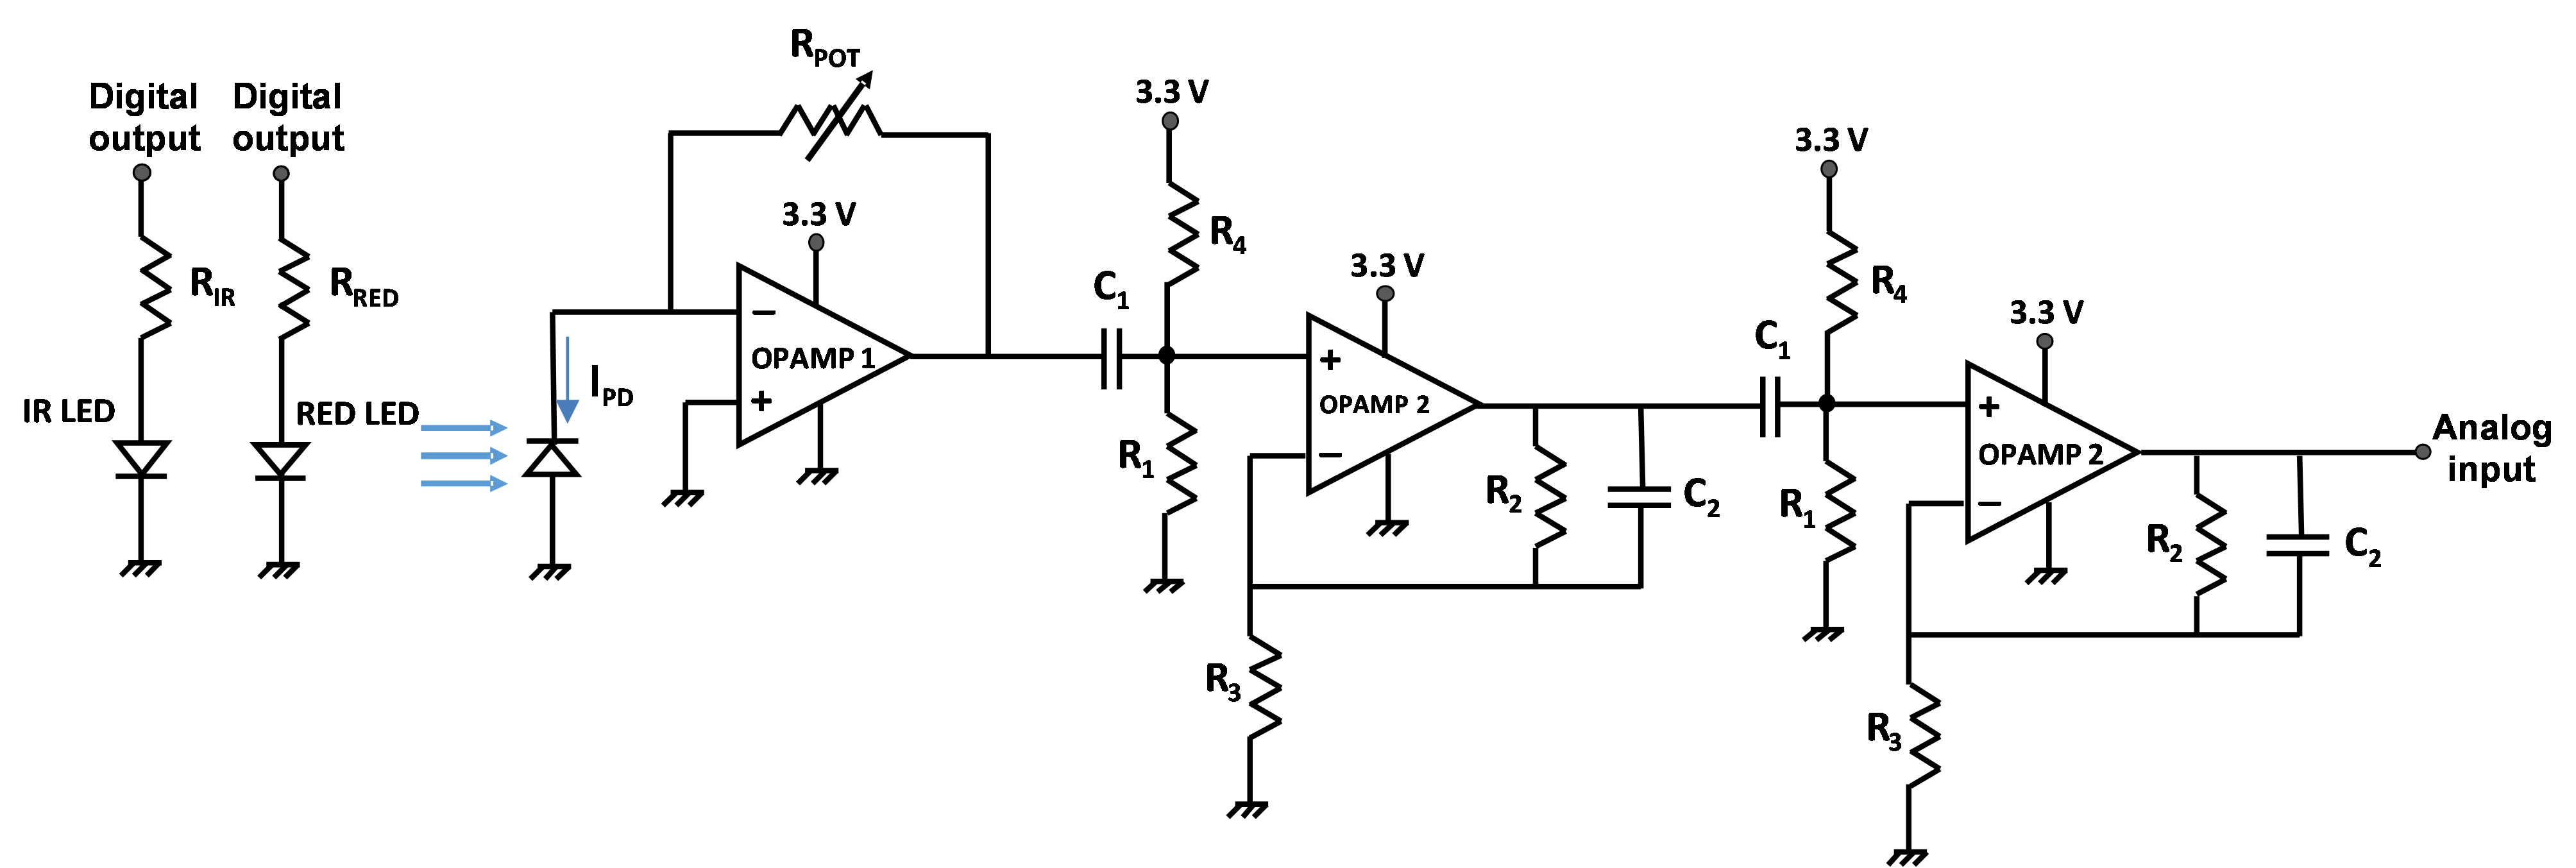
\includegraphics[width=\linewidth]{Circuit1.png}
    \caption{Schema circuito }
    \label{fig:Circuit}
\end{figure}
Il circuito è alimentato mediante porta USB del PC, la quale eroga circa $(\sim 5 V)$. Ed è composto da un primo stadio (OPAMP 1) "in cui si va a regolare l'offset" e un secondo stadio in cui vi è un doppio filtro passa-banda (OPAMP 2) che taglia le frequenze inferiori a 0.8 Hz e superiori a 3 Hz.
\subsection{Dimensionamento resistenze LED}
Dimensioniamo le resistenze $R_{IR},R_{RED}$ in modo da ottenere sui due LED rosso e infrarosso, correnti pari a $I_{RED}=15\text{ mA},I_{IR}=$3 mA rispettivamente. Usando i pin high current della scheda Arduino Due che riescono riescono ad erogare una corrente massima di 15 mA
\begin{equation}
    \frac{V_{CC}-V_{f,IR}}{I_{IR}}=100\text{ }\Omega\quad\frac{V_{CC}-V_{f,RED}}{I_{RED}}=103.33\text{ }\Omega
\end{equation}
Dove i valori della tensione di Forward lì abbiamo reperiti dal datasheet e valgono $V_{f,IR}=3$ V e $V_{f,RED}=1.75$ V.
\subsection{Calcolo funzioni di trasferimento}
Calcoliamo ora la funzione di trasferimento del
\begin{itemize}
    \item Filtro passa-alto costituito da $C_1,R_1,R_4$
    \item Filtro passa-basso costituito da $C_2,R_2,R_3$
    \item Filtro passa-banda complessiva
\end{itemize}
\subsection{Dimensionamento resistenze filtro}
Dimensioniamo le resistenze $R_1, R_2, R_3, R_4$ in modo da ottenere:
\begin{itemize}
    \item Il filtro passa-alto costituito da $C_1, R_1, R_4$ abbia frequenza di taglio pari a 0.8 Hz
    \item La tensione DC a riposo ai morsetti $V_+$ sia pari a 0.15 V
    \item Il filtro passa-basso costituito da $R_2, R_3, C_2$ abbia frequenza di taglio pari a 3 Hz
    \item Il guadagno in DC del filtro passa-basso costituito da $R_2, R_3, C_2$ sia pari a 11   
\end{itemize}
Sceglieremo poi il valore commerciale più vicino per le resistenze $R_1, R_2, R_3, R_4$
\subsection{Tracciamento risposta in frequenza filtro}
Con i valori scelti al punto \ref{}, tracciamo la risposta in frequenza di:
\begin{itemize}
    \item Filtro passa-alto costituito da $C_1,R_1,R_4$
    \item Filtro passa-basso costituito da $C_2,R_2,R_3$
    \item Filtro passa-banda complessiva
\end{itemize}
evidenziando le frequenze di taglio ottenute utilizzando i valori commerciali delle resistenze, necessariamente diverse da 0.8 Hz e 3 Hz
    \clearpage
    
    \section{Stadio digitale Arduino}
    Dopo aver montato il circuito in Figura \ref{fig:Circuit}, connettiamo il segnale $V_0$ all'ingresso analogico A0 della scheda Arduino Due. Utilizziamo la scheda custom contenente fotodiodo VIS/IR e diodo LED IR mostrata nella Figura \ref{fig:HRS}, utilizzando il datasheet dei componenti per definire la polarità degli stessi.
\begin{figure}[H]
    \centering
    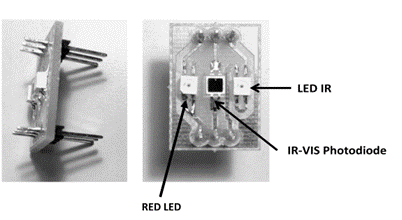
\includegraphics[width=0.5\linewidth]{Sensor.png}
    \caption{Heart Rate Sensor}
    \label{fig:HRS}
\end{figure}
Per l'analisi della frequenza cardiaca utilizziamo solamente il LED infrarosso.
\subsection{Codice acquisizione}
Scrivere un codice che permetta di acquisire il segnale in uscita al cardiofrequenzimetro, graficandolo sul display TFT allo stesso tempo. Si utilizzi per il momento il LED infrarosso per questa analisi
\begin{lstlisting}[frame=single, language=Arduino]
#include <SPI.h>
#include "Adafruit_GFX.h"
#include "Adafruit_HX8357.h"

#define sensorPin A0
#define PinIR 12
#define PinRED 11
#define TFT_CS 10
#define TFT_DC 9

Adafruit_HX8357 tft = Adafruit_HX8357(TFT_CS, TFT_DC,-1); 

const int displayWidth = 480;
const int arraySize = displayWidth;
const int graphHeight = 200;
const int sampleInterval = 20;

int acquire[arraySize];
\end{lstlisting}
\clearpage
\begin{lstlisting}[frame=single, language=Arduino]
void setup(){
    pinMode(PinIR,OUPUT);
    pinMode(PinRED,OUTPUT);
    analogReadResolution(12); // 12 bit ADC -> 4096 values

    tft.begin();
    tft.setRotation(3);
    tft.fillScreen(HX8357_BLACK);
    tft.setTextSize(3);
    tft.setCursor(30, graphHeight);
    tft.setTextColor(HX8357_WHITE);
    tft.println("Heart Rate Monitor");
}

void loop(){
    tft.setCursor(30, 240);
    tft.setTextColor(HX8357_WHITE);
    digitalWrite(PinIR,HIGH);
    tft.print("Inizio misurazione ...");    delay(1000);    
    tft.print("3"); delay(1000);    
    tft.print("2"); delay(1000);    
    tft.print("1"); delay(1000);
    tft.fillRect(0, 240, displayWidth, 80, HX8357_BLACK);
    acq();
    digitalWrite(PinIR,LOW);
    tft.setCursor(30, 240);
    tft.print("Scalamento della misurazione ...");
    plot_array_scaled(acquire);
    tft.fillRect(0, 240, displayWidth, 80, HX8357_BLACK);
}
\end{lstlisting}
\begin{lstlisting}[frame=single, language=Arduino]
void acq(){
    unsigned long currentMillis = 0;
    tft.fillRect(0, 0, displayWidth, graphHeight, HX8357_BLACK);
    for(int i = 0; i < arraySize; i++){
        acquire[i] = analogRead(sensorPin);
        currentMillis = millis();
        tft.drawPixel(i, map(array[i], 0, 4095, 0, graphHeight), HX8357_WHITE);
        while(millis() < currentMillis + sampleInterval);
    }
}
\end{lstlisting}
\subsection{Codice plotting}
Una volta acquisito l’array di valori, interrompere l’acquisizione. Scrivere una funzione che ri-scali l’array in modo di visualizzarlo sula metà superiore dello schermo, insieme ad eventuali altre scritte (v. esempio in figura); riportare sotto il corrispondente codice
\begin{lstlisting}[frame=single, language=Arduino]
void plot_array_scaled(int array[]){
    rescale();
    tft.fillRect(0, 0, displayWidth, graphHeight, HX8357_BLACK);
    for(int i = 0; i < arraySize; i++){
        tft.drawPixel(i, array[i], HX8357_WHITE);
    }
}
void rescale(){
    int max = findmax(acquire);
    int min = findmin(acquire);

    for(int i = 0; i < arraySize; i++){
        acquire[i] = map(acquire[i], min, max, 0, graphHeight);
    }
}

int findmax(int array[]){
    int max = array[0];
    for(int i = 0; i < arraySize; i++){
        if(array[i] > max)  max = array[i];
    }
    return max;
}

int findmin(int array[]){
    int min = array[0];
    for(int i = 0; i < arraySize; i++){
        if(array[i] < min)  min = array[i];
    }
    return min;
}
\end{lstlisting}    
    \section{Misura dei BPM}
    A partire dall’array acquisito, scrivere un codice che permetta di misurare la frequenza cardiaca e visualizzarne il corrispondente valore sul display
\begin{lstlisting}[frame=single, language=Arduino]
int findBPM(int array[]){
    int min = findmin(array);
    int threshold = (findmax(array) - min) / 1.5 + min;
    int peaks = 0;
    int timeOfPeaks[arraySize/2];
    for(int i = 0; i < arraySize; i++){
        if(array[i] > threshold){
            timeOfPeaks[peaks] = i;
            peaks++;
            i+=2;
            while(array[i] > threshold){
                i++;
            }
        }
    }
    FistPeaks = timeOfPeaks[0] * 20;
    LastPeaks = timeOfPeaks[peaks-1] * 20;

    TimeInterval = LastPeaks - FirstPeaks; // in microseconds
    
    return peaks / ((TimeInterval) / 60000);
}
\end{lstlisting}    
    \section{Misura saturazione $O_2$}
    Scrivere il codice che permette di misurare la concentrazione di ossigeno nel sangue, valutando il rapporto R tra l’assorbimento della componente rossa e infrarossa, secondo la formula seguente
\begin{equation}
    R=\frac{\left(\frac{AC}{DC}\right)_{RED}}{\left(\frac{AC}{DC}\right)_{IR}}=\frac{\frac{\left(V_{\text{max},RED}-V_{\text{min},RED}\right)}{V_{\text{min},RED}}}{\frac{\left(V_{\text{max},IR}-V_{\text{min},IR}\right)}{V_{\text{min},IR}}}
\end{equation}
A partire da R, è possibile calcolare il livello di saturazione utilizzando la formula riportata in Figura \ref{fig:GraphO2}
\begin{figure}[H]
    \centering
    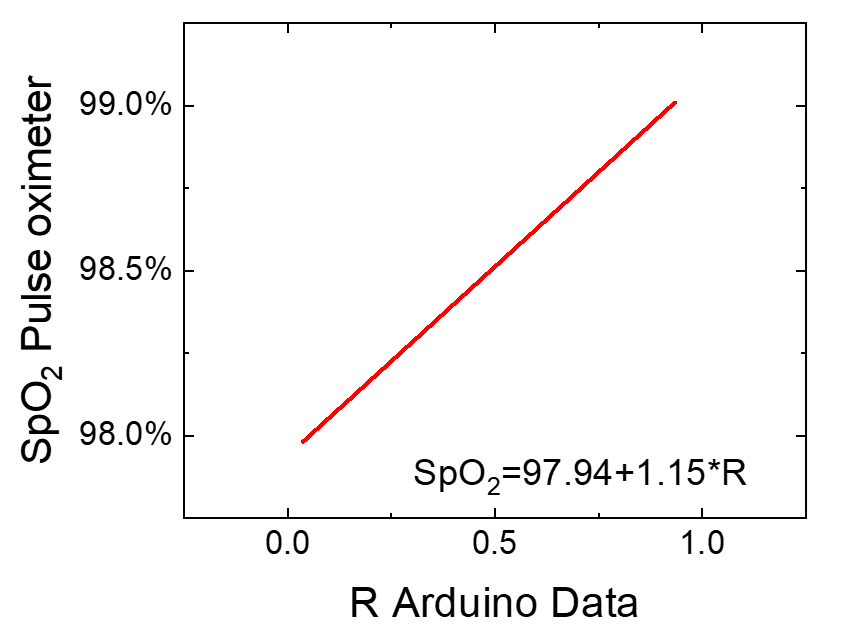
\includegraphics[width=0.7\linewidth]{GraphO2.png}
    \caption{$SpO_2$ pulse oximeter}
    \label{fig:GraphO2}
\end{figure}
\begin{lstlisting}[frame=single, language=Arduino]
float findO2(int array[]){
    int samples = 1000;
    int IR[samples];
    int RED[samples];
    digitalWrite(PinIR,HIGH);
    delay(250);
    for(int i = 0; i < samples; i++){
        IR[i] = analogRead(sensorPin);
        delay(1);
    }
    digitalWrite(PinIR,LOW);
    delay(100);
    digitalWrite(PinRED,HIGH);
    delay(250);
    for(int i = 0; i < samples; i++){
        RED[i] = analogRead(sensorPin);
        delay(1);
    }
    digitalWrite(PinRED,LOW);

    int IRmax = findmax(IR) * 3.3 / 4095;
    int IRmin = findmin(IR) * 3.3 / 4095;
    int REDmax = findmax(RED) * 3.3 / 4095;
    int REDmin = findmin(RED) * 3.3 / 4095; 

    float R = ((REDmax - REDmin)/REDmin) / ((IRmax - IRmin) / IRmin);
    float O2 = 97.94 + 1.15 * R;

    return O2;
}
\end{lstlisting}
    \section{Foto del display}
    Si conclude con una foto del display HX8357 Adafruit, scattata al termine dell'esperienza

\begin{figure}[H]
    \centering
    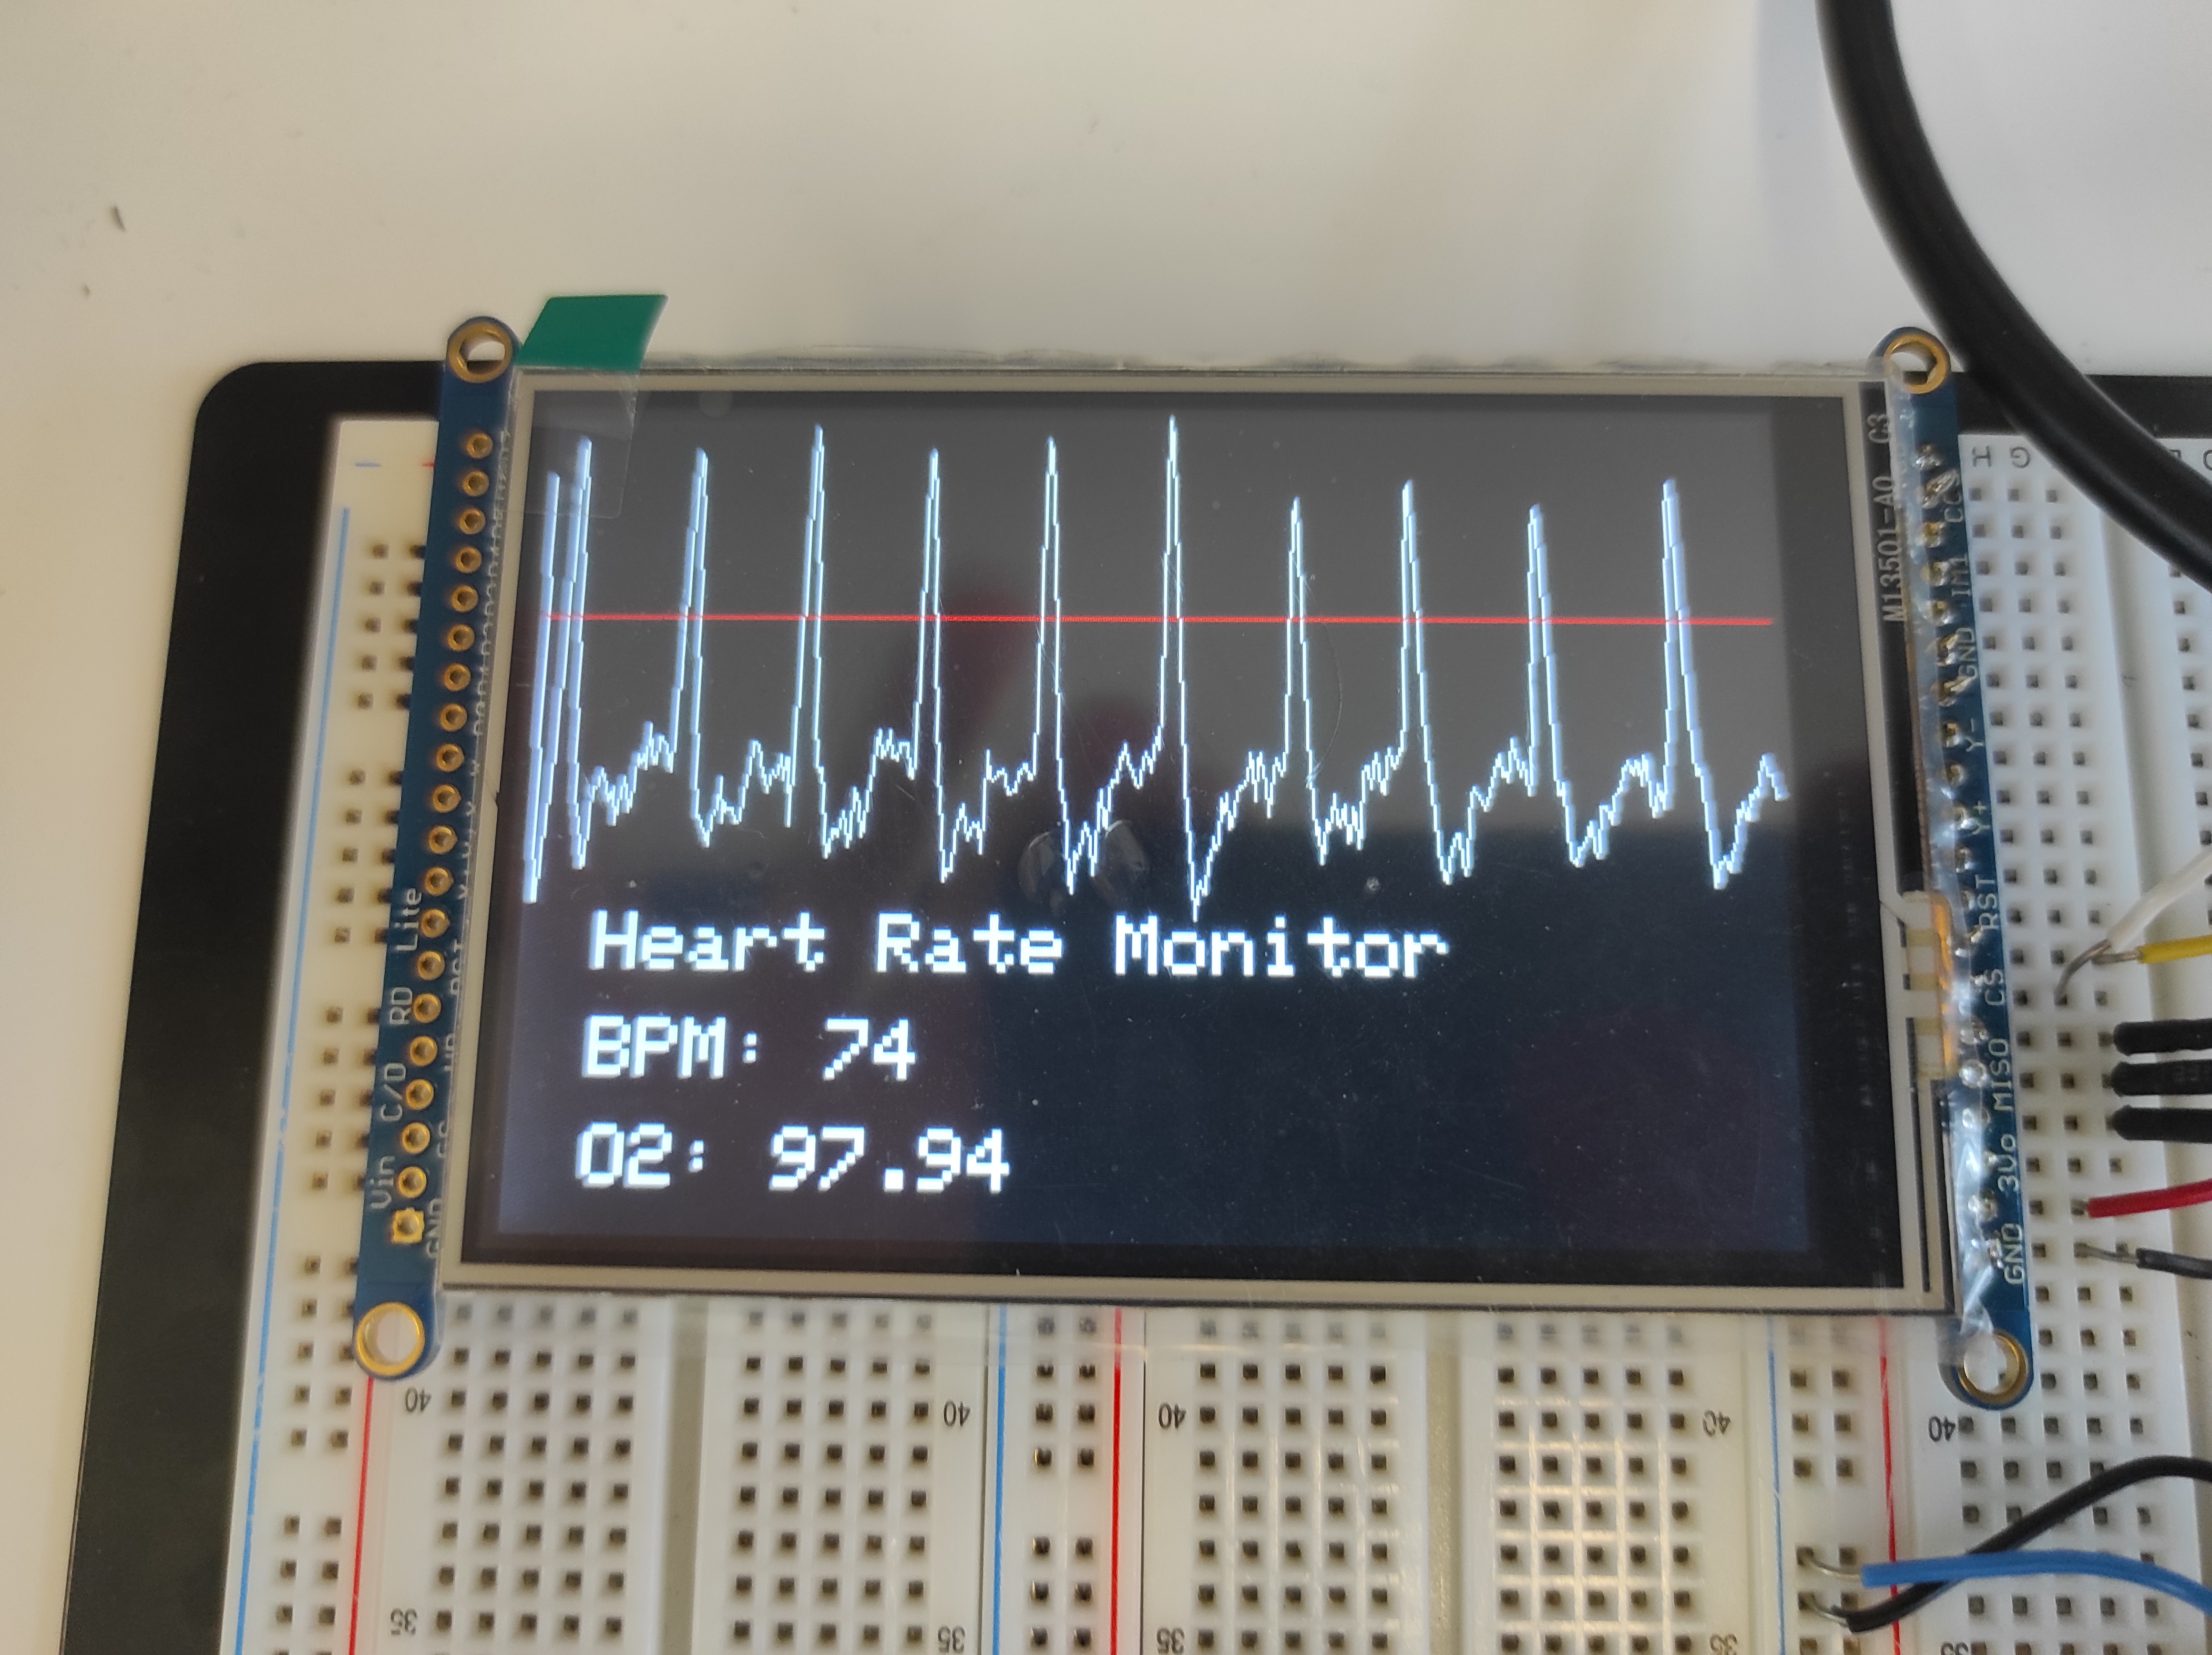
\includegraphics[width=0.7\linewidth]{IMG_20230526_120648.jpg}
    \caption{Foto del Display HX8357}
    \label{fig:IMG_20230526_120648}
\end{figure}
\end{document}
